\documentclass[12pt]{article}
\usepackage[utf8]{inputenc}
\usepackage{amsmath}
\usepackage{physics}
\usepackage{graphicx}
\usepackage{float}

\begin{document}

The model tells us that production is linear in time, or that the rate of production is constant, and that the number of viable sperm decays over time at some rate. This is modeled by the differential equation
\begin{eqnarray*}
    \dv{N}{t} = R - kN
\end{eqnarray*}

We can analytically solve for the maximum number of sperm given a linear roproduction rate and exponential decay rate:
\begin{align*}
\dv{N}{t} = 0 \Rightarrow N = \frac{R}{k}
\end{align*}

This informs us about whether a person is capable of producing enough sperm to be able to likely reproduce without much trouble, where the critical value is about 15 million sperm per milliliter. We can also plug in different rates and evolve the state from the differential equation above and observe how many sperm are present. Then, we must simply divide by the volume of the ejaculate to determine if the density is large enough.

We use the Runge-Kutta method to solve the system, which is summarized below:
\begin{align*}
\begin{cases}
t_{n+1} = t_n + \Delta t \\
N_{n+1} = N_n + \frac{1}{6}\qty(k_1 + k_2 + k_3 + k_4)
\end{cases}
\end{align*}
where
\begin{align*}
\begin{cases}
k_1 = \Delta t f(N_n) \\
k_2 = \Delta t f(N_n + \frac{k_1}{2}) \\
k_3 = \Delta t f(N_n + \frac{k_2}{2}) \\
k_4 = \Delta t f(N_n + k_3)
\end{cases}
\end{align*}

The following plots show the results of the simulations. Note that a standard initial condition of $N(0) = 0$ was used for all simulations.

For the first plot we use a reproduction rate of 1500 sperm per second, which is reported by many sources online as an average male sperm cell reproduction rate. The different lines come from half life values of 5 days, 2 days, and 8 hours. As expected, if the half-life decreases the sperm reproduction slows more quickly over time and reaches a smaller maximum value.

\begin{figure}[H]
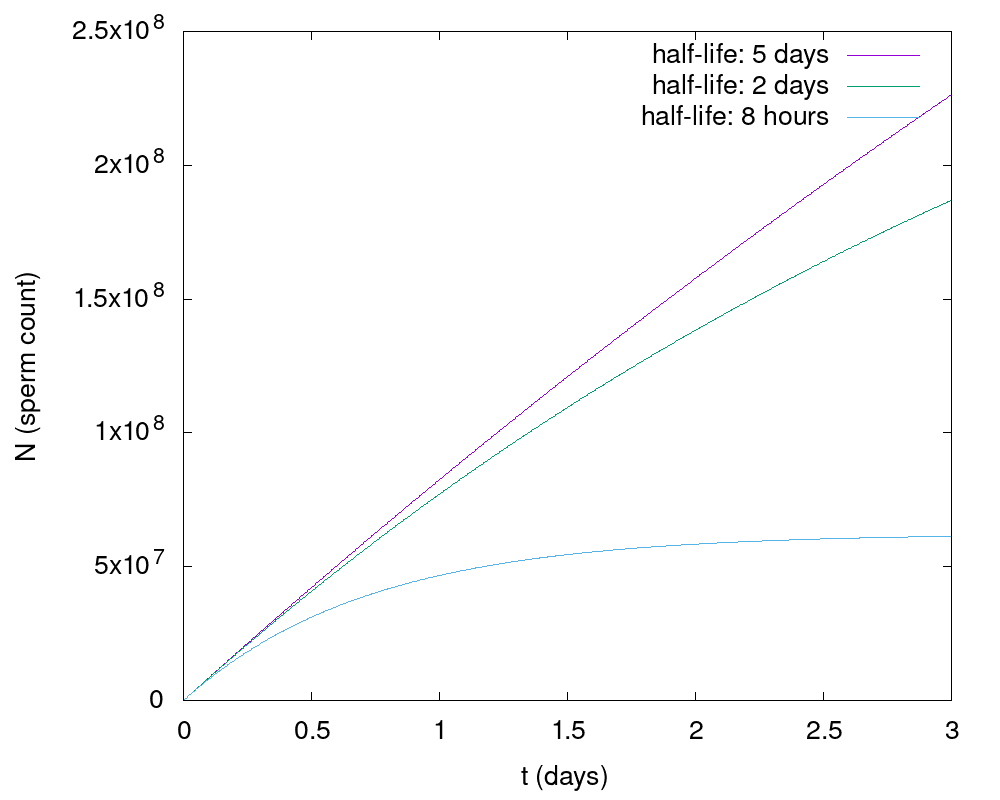
\includegraphics[scale=0.5]{./output.png}
\end{figure}

Next, we use a standard half-life of 5 days and alter the reproduction rate between 1500, 500, and 100 sperm per second. It is seen that smaller maxima are reached if the rate is lower, as expected.

\begin{figure}[H] 
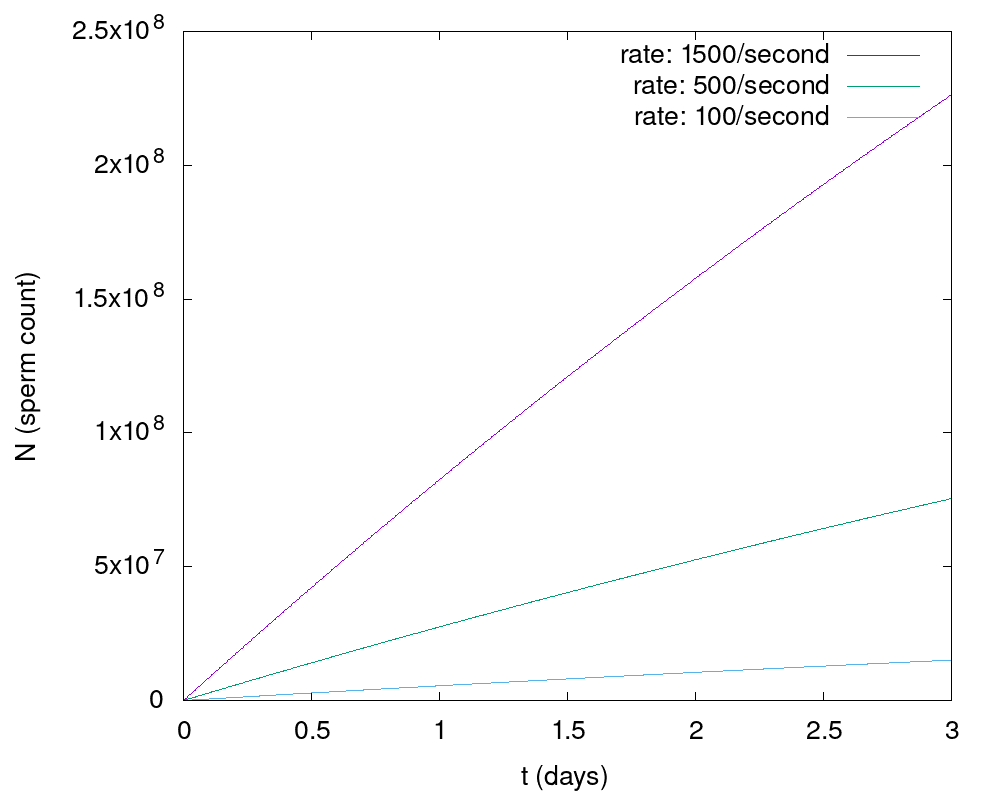
\includegraphics[scale=0.5]{./output1.png}
\end{figure}



\end{document}
